\label{sec:hadronictrigger}
Searches for SUSY at the LHC typically suppress the overwhelming QCD background by requiring events to have a large $\met$ as a criterion for firing the trigger. Additionally, for searches in the hadronic channel, a minimum amount of $\Ht$ can also be required, or some combination of $\met$ and $\Ht$. Hadronic searches typically collect data using triggers that accept events (fire) if these observables exceed some threshold. However, because online calculations must be performed rapidly, only rough approximations of the $\Ht$ and $\met$ can be obtained in real time. Therefore, substantial discrepancies can arise between the online objects and the more precise offline objects, since the latter benefit from the availability of greater computing resources. In order to guarantee that a trigger fire on an event with a desired offline $\met$, the online $\met$ threshold must be sufficiently lower than the offline $\met$ threshold. This introduces the concept of a trigger turn-on curve, which is the nickname for the trigger efficiency, that is, the probability of the trigger firing, as a function of an offline variable. $\met$ trigger turn-on curves have notoriously gradual slopes, because the calculation of the $\met$ is particularly sensitive to jet energy resolutions, which differ substantially in the offline and online event reconstruction.

Two conditions must be met in order for a trigger to be useful. First, the trigger must have a sufficiently high efficiency for selecting signal events. And second, it must be possible to make an unbiased measurement of the trigger efficiency. The former is typically a matter of choosing an appropriate trigger. For the latter, it is best to measure the trigger efficiency using real data, but in order to do so without bias, one needs a sample of events, referred to as a reference sample, that is independent of the events that pass the trigger. 

\subsection{Measuring the efficiency without bias}
Suppose the goal is to make a measurement of the efficiency of trigger A. One can make an unbiased measurement by obtaining a sample of events collected by trigger B, so long as the absolute probability of firing trigger A, P(A), is equal to the conditional probability of trigger A firing given that trigger B has also fired, P(A$|$B):
\begin{equation}
\text{P(A)} = \text{P(A|B)}.
\label{eq:trigcondition}
\end{equation}
In other words, trigger B should be chosen such that its triggering criteria are independent of those of trigger A. Whether or not Equation \ref{eq:trigcondition} holds can be by simulating the triggers. Finally, the unbiased estimate of the efficiency of trigger A is the fraction of events that fire trigger B that also fire trigger A:
\begin{equation}
\hat{\epsilon}_{\text{A}} = \frac{N_{\text{fire A and B}}}{N_{\text{fire B}}}.
\label{eq:trigeff}
\end{equation}
This is an estimate of P(A|B) with an expectation value equal to P(A) if, and only if, P(AB) = P(A)P(B), that is triggers A and B are independent.

One might choose to collect data using the trigger named
\begin{itemize}
  \item \texttt{HLT\_PFMETNoMu90\_PFMHTNoMu90},
\end{itemize}
referred to as the monojet trigger. Here, PFMET and PFMHT refer to the online $\met$ and $\mht$ computed using the particle flow (PF) algorithm (Section \ref{sec:reconstruction}), NoMu refers to the fact that muons are neglected in the online computation of these observables, and the number 90 refers to the triggering thresholds in units of GeV. The trigger efficiency must be estimated as a function of the offline $\Ht$ and $\mht$. In this example, the monojet trigger is treated as trigger A above. 

Trigger B, or the reference trigger, is chosen to be the trigger named
\begin{itemize}
  \item \texttt{HLT\_Ele27\_eta2p1\_WPLoose\_Gsf\_v*}, 
\end{itemize}
which selects events that contain an electron reconstructed by the GSF algorithm (Section \ref{sec:reconstruction}) with a $\pt$ greater than 27 GeV and pseudorapidity less than than 2.1,
and take the base sample to be the subset of these events that have $\text{N}_{\text{jets}}>3$ and a single offline reconstructed electron.  

A sample of simulated t$\bar{\text{t}}$ events is used to establish the validity of Equation \ref{eq:trigcondition}. First, the conditional probability of firing the primary trigger, given that the reference trigger fired, is computed as a function of the offline $\Ht$ and $\mht$. Then, the absolute probability of firing the primary trigger is computed by replacing the reference sample with the entire sample of simulated events, as a function of the same variables. The ratio of the conditional probability (``method'') to the absolute probability (``truth'') is shown in Fig. \ref{fig:2dEffRatio}. 
\begin{figure}[tb!]
  \begin{center}
    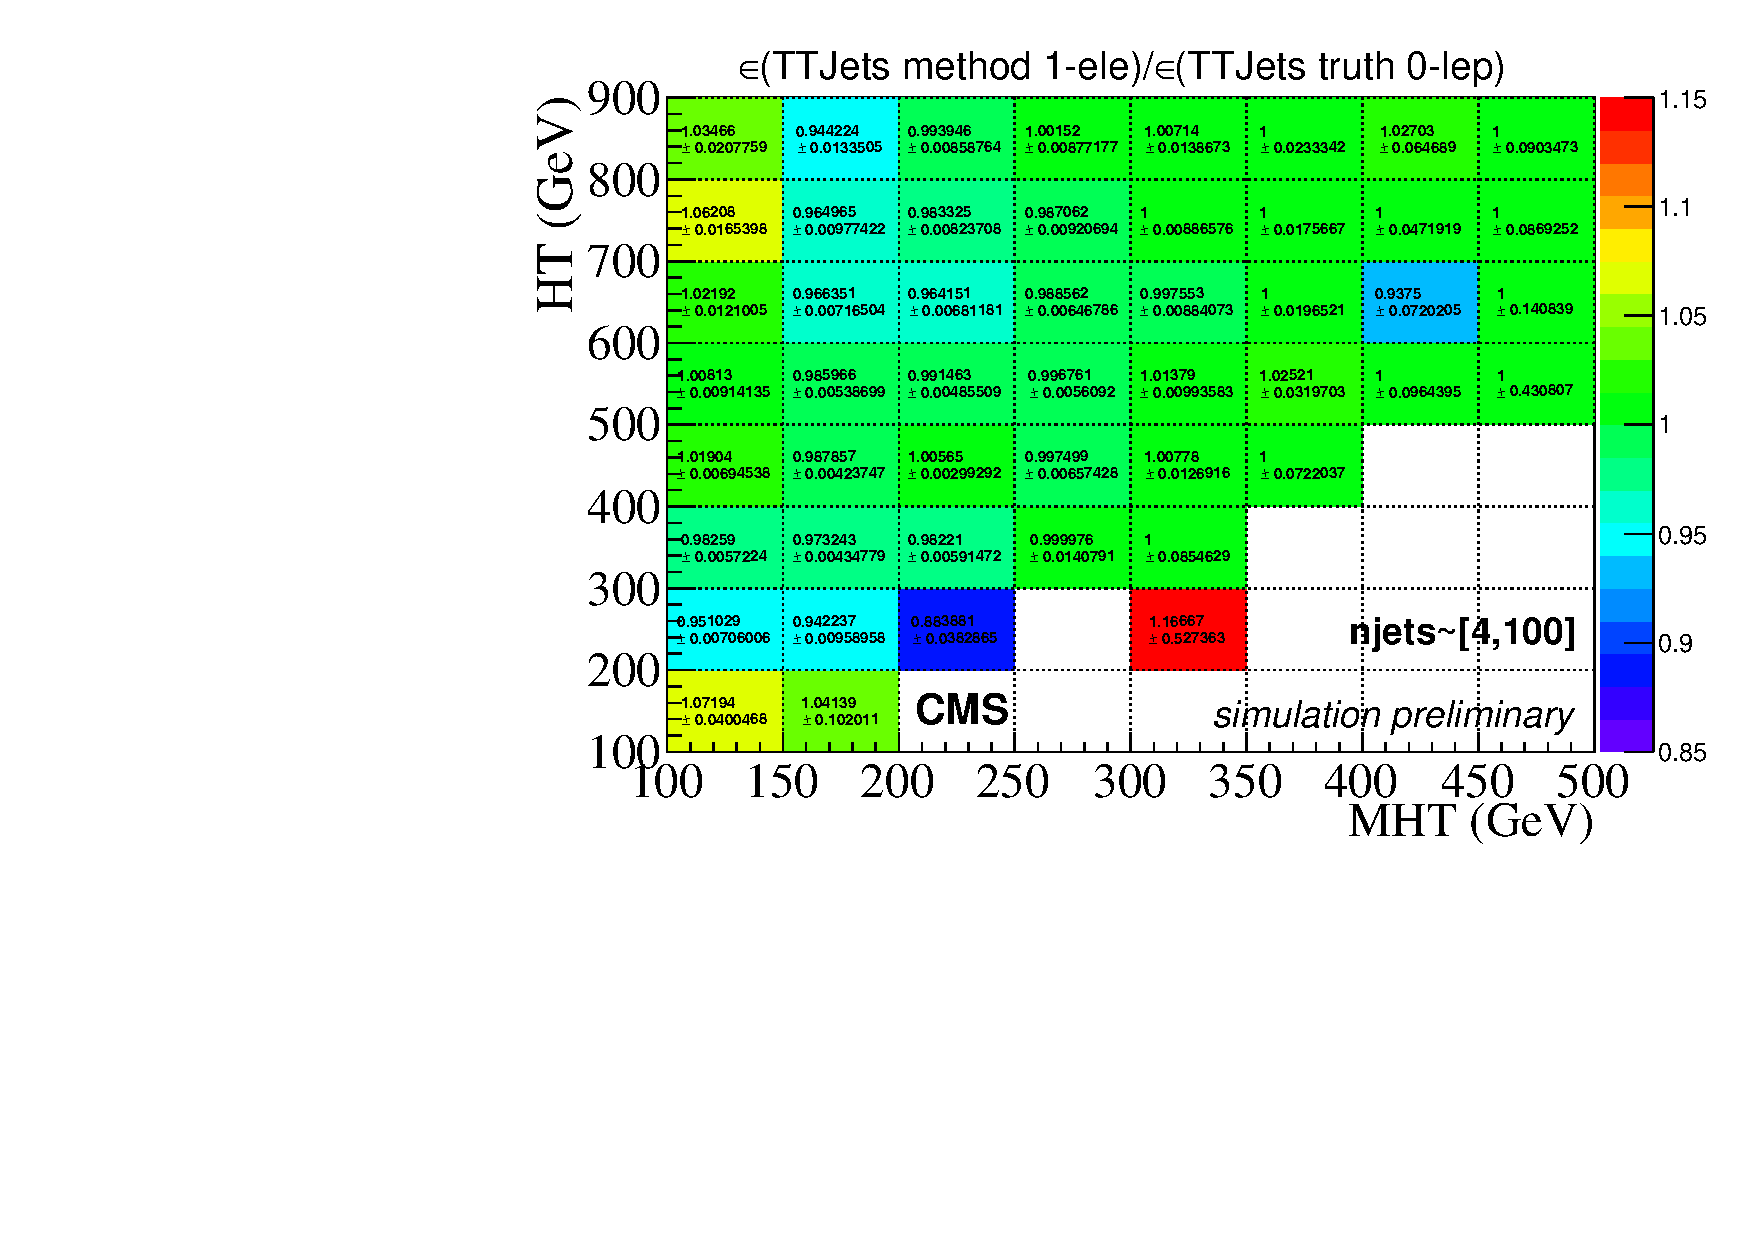
\includegraphics[width=0.95\linewidth]{figures/trigger/MonojetTrigger_EfficiencyRatioMC.pdf}
    \caption{
      The ratio of the monojet trigger efficiency for events passing the single
      electron reference trigger to the trigger efficiency for all
      events in a simulated t$\bar{\text{t}}$ sample, as a function of the offline $\Ht$
      and $\mht$. The ratio is consistent with 1 throughout the $\Ht-\mht$ plane.}
    \label{fig:2dMonoEffRatio}
  \end{center}
\end{figure}

The primary and reference triggers have been shown to satisfy Equation \ref{eq:trigcondition}, so there is now license to measure the trigger efficiency in real data.  Figure \ref{fig:2dMonoEff} shows the efficiency, computed using Equation \ref{eq:trigeff}. The efficiency is nearly 1 for kinematic regions with $\mht>200$ GeV, making the monojet trigger an ideal choice for a hadronic searches for physics in the low-$\Ht$ region.

\begin{figure}[tb!]
  \begin{center}
    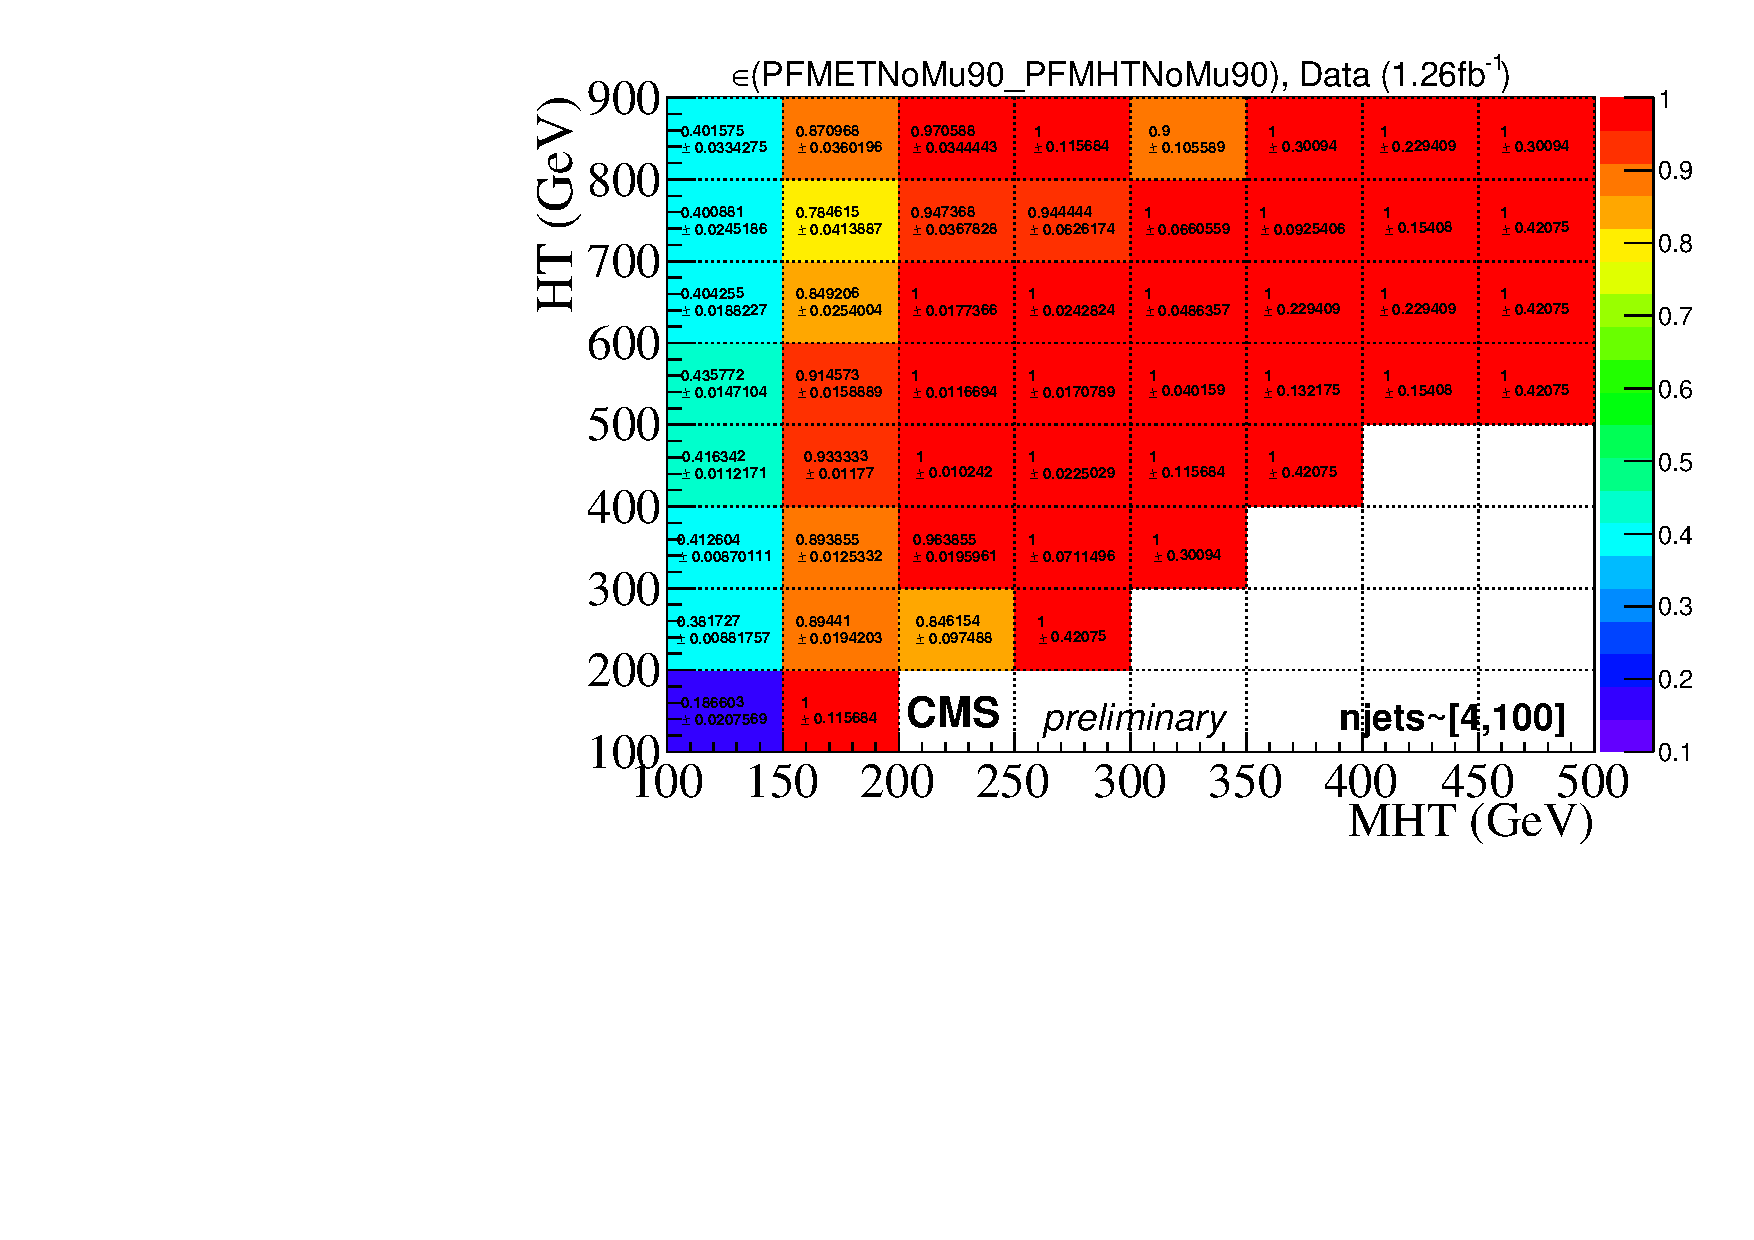
\includegraphics[width=0.95\linewidth]{figures/trigger/MonojetTrigger_EfficiencyData.pdf}
    \caption{
      The monojet trigger efficiency, measured in real data, as a function of the offline $\Ht$
      and $\mht$. }
    \label{fig:2dMonoEff}
  \end{center}
\end{figure}


If the condition in \ref{eq:trigcondition} is found not to hold for a particular reference trigger, the efficiency can still be measured, but a systematic uncertainty must be applied to the estimate of the efficiency to account for the bias. These systematic uncertainties can typically be reduced or eliminated by more intelligently choosing a set of observables on which the efficiency estimation depends, in this case the $\Ht$ and $\mht$. This is discussed below under the subsection heading ``Multivariate trigger techniques,'' in the context of more advanced techniques for determining the trigger efficiency. 
 
\subsection{Multivariate classification}
\label{sec:mvatrigger}
It is possible for the trigger efficiency to vary as a complicated function of the observables in events. Often, a trigger decision involves a long chain of HLT (Chapter \ref{chap:cms} Section \ref{sec:Trigger}) modules, or filters, that can potentially induce unforeseen dependencies of the probability of firing the trigger on non-trivial correlations among the observables. One way to account for these correlations is to increase the dimensionality of the parametrization of the trigger efficiency estimation. For example, the jet multiplicity could be added as a third parameter to accompany the previously described $\Ht$ and $\mht$ parameterization if it were believed that $\njets$ were a determinant of the efficiency. However, adding additional dimensions requires the division of the event sample into a larger number of bins, which reduces the counts in each bin. This approach is ultimately plagued by the curse of dimensionality.

It is possible to reduce the dimensionality of the parametrization to just 1 dimension by constructing an appropriate single-valued function of the relevant observables. Such a function can be obtained through the use of a Bayesian neural network (NN) classifier, as previously demonstrated in the context of b-tagging triggers \cite{bib:SezenTrigger}. 

As stated in Equation \ref{eq:mlp}, the output of such a classifier can be interpreted as
\begin{equation}
\text{NN} = P(\text{s}|\vec{\theta}) = \frac{p(\vec{\theta} | {\rm s})}{p(\vec{\theta} | {\rm s})+p(\vec{\theta} | {\rm b})},
\end{equation}
where $\vec{\theta}$ is a vector of observed quantities, also called the data, and s and b are, respectively, the true and false outcomes\textemdash in this case, the decision made by the trigger to fire or not. Since a NN is capable of training with a vector $\theta$ of arbitrary length, it is worth including any observable that may be relevant for the determination of the efficiency. To train the NN for the monojet trigger efficiency, the single electron reference sample is divided into events that fire the monojet trigger, which serve as the signal training events, and events that fail the monojet trigger, which serve as the background training events. There are several internal NN parameters, which govern aspects of the output such as the responsiveness of the output to small fluctuations in the data. These parameters are assigned gaussian prior probability densities that are broad distributions relative to the likelihood functions, which are highly corrugated, a combination that results in posterior densities for the NN parameters being dominated by the likelihoods. To obtain an uncertainty in the efficiency estimate, the posterior densities of the NN parameters are randomly sampled, and an ensemble of efficiency estimates are obtained. The mode of the envelope of this ensemble defines the central efficiency estimate, and the uncertainty band taken as the interval that is centered on the mode and contains 68\% of the estimated efficiency values. 

Figure \ref{fig:mvatrigger} shows the dependence of the monojet trigger efficiency on a few kinematic variables, both for the NN-derived efficiency and the efficiency computed in the traditional way. As values of the $\Ht$ are scanned over, the NN efficiency reveals a dependence on correlations between the $\Ht$ and $\mht$. Importantly, this manifests as the loss of efficiency for very high $\Ht$ around $\mht\approx200-300$ GeV. Traditional, binned efficiency measurements may easily hide such inefficiencies, particularly if regions with low efficiency are combined with  regions of maximum efficiency. The NN method provides is a natural way to avoid bias associated with binned efficiency estimates. 
\begin{figure}[tb!]
  \begin{center}
    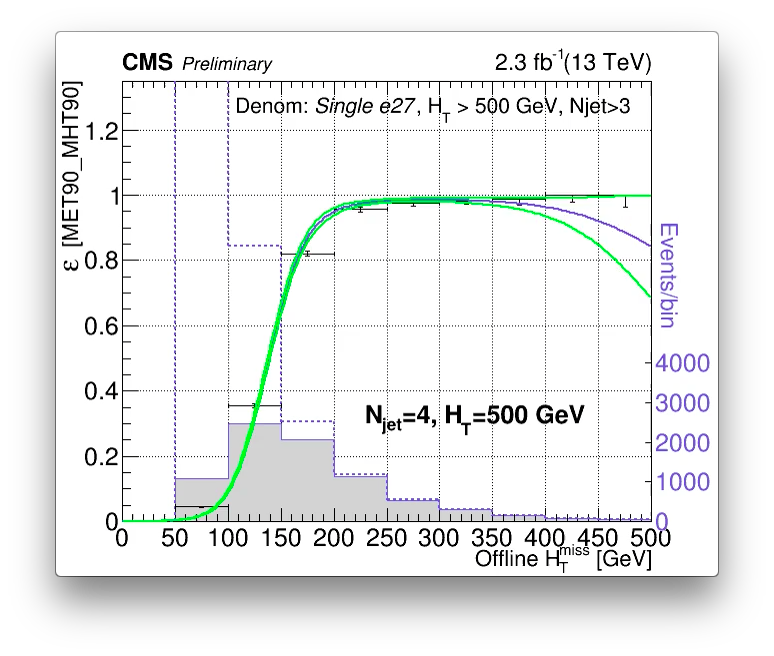
\includegraphics[width=0.49\linewidth]{figures/trigger/MonoTrigEff_Ht500.png}
    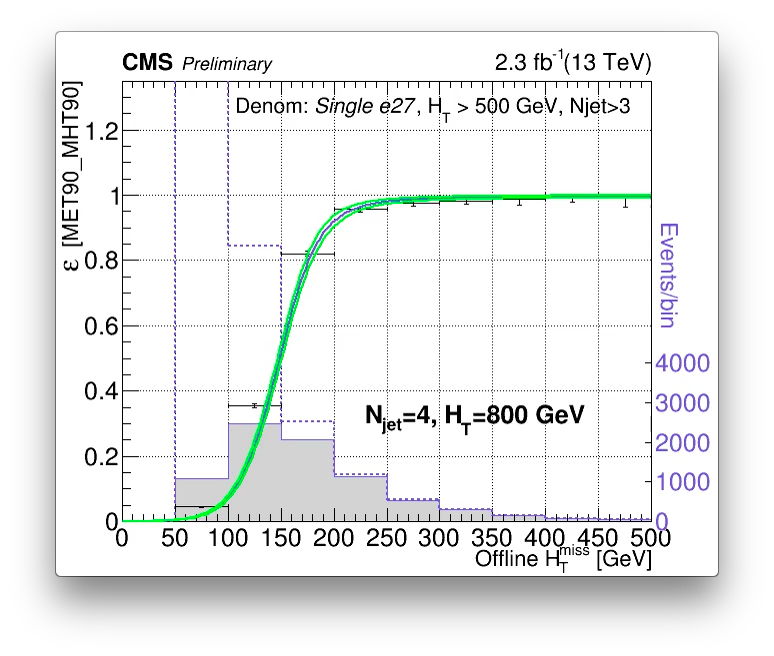
\includegraphics[width=0.49\linewidth]{figures/trigger/MonoTrigEff_Ht800.png}\\
        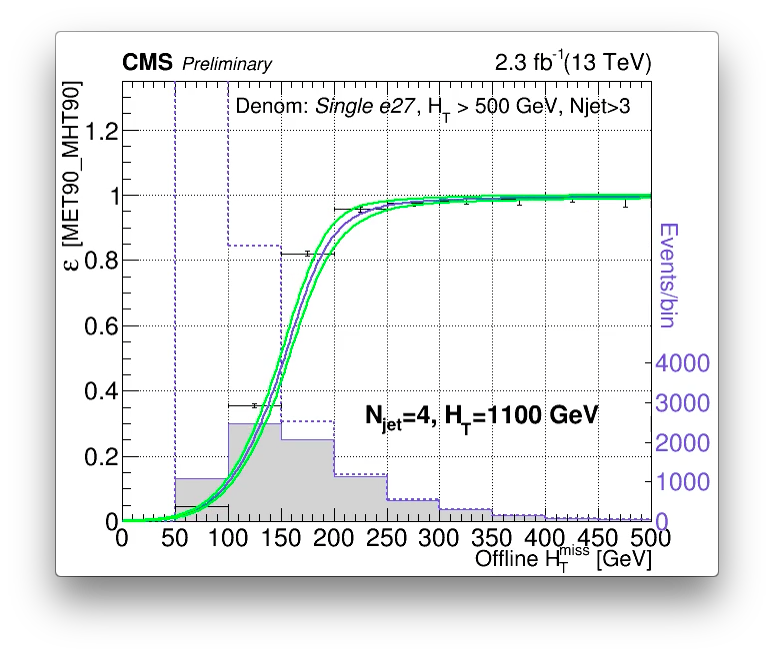
\includegraphics[width=0.49\linewidth]{figures/trigger/MonoTrigEff_Ht1100.png}
    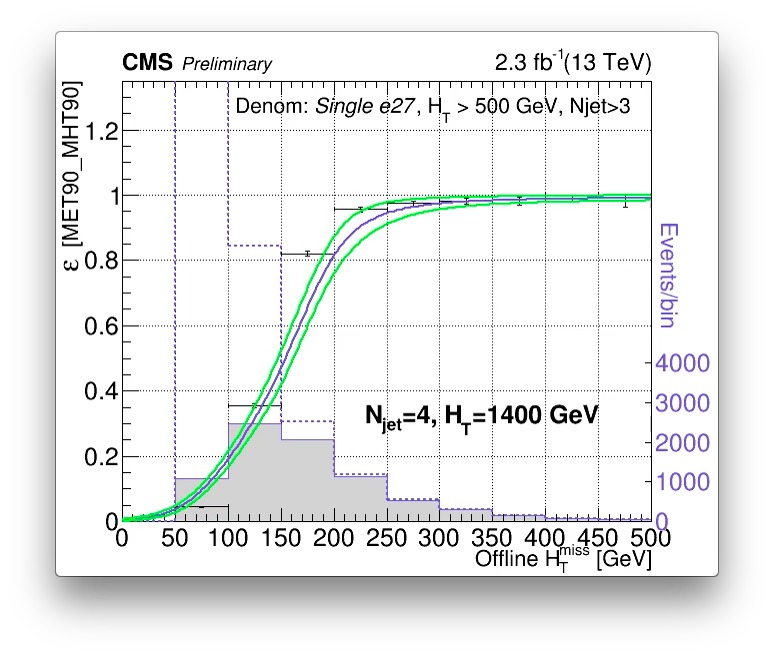
\includegraphics[width=0.49\linewidth]{figures/trigger/MonoTrigEff_Ht1400.png}\\
        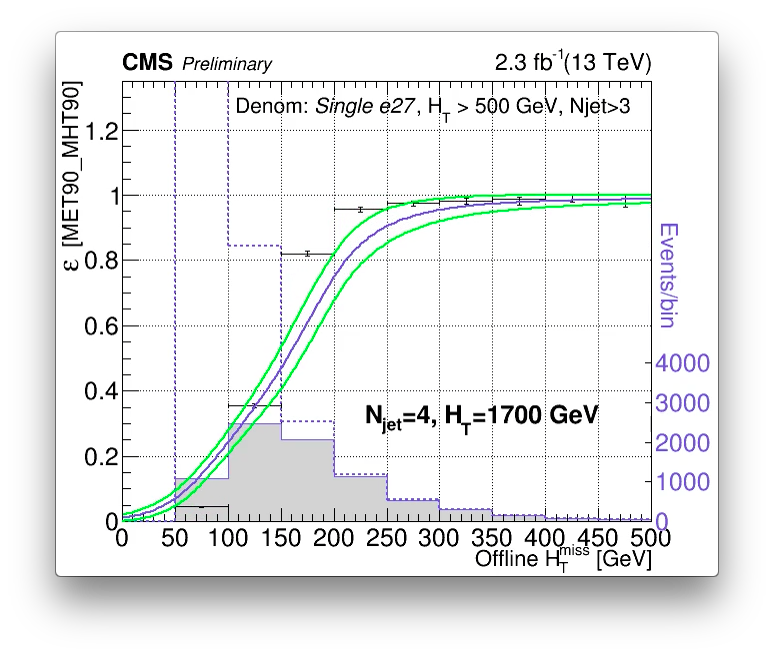
\includegraphics[width=0.49\linewidth]{figures/trigger/MonoTrigEff_Ht1700.png}
    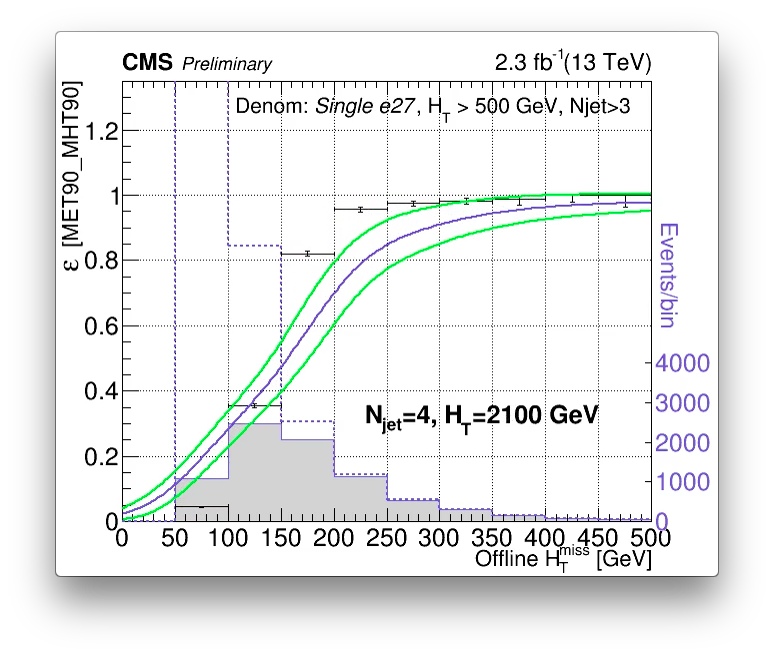
\includegraphics[width=0.49\linewidth]{figures/trigger/MonoTrigEff_Ht2100.png}
    \caption{The trigger efficiency as a function of the offline $\mht$ for the monojet trigger, measured the traditional way (histograms) and by the NN method (blue function), for $\njets=4$, with varying values of the $\Ht$. The green function lines show the 1-sigma uncertainty on the efficiency. }
    \label{fig:mvatrigger}
  \end{center}
\end{figure}
\noindent

This method is particularly well-suited for analyses that consider events in regions of kinematic phase space in which the trigger efficiency is varying as a function of the observables.  Typically, analyses avoid such regions, since traditional trigger efficiency estimation techniques can hide potentially detrimental effects in these regions, such as the efficiency loss at high $\Ht$ revealed in Fig. \ref{fig:mvatrigger}. Such kinematic regions include the low to moderate $\Ht$ and $\mht$ regions, which were identified as potentially signal rich in Chapter \ref{chap:run1pmssm}.
